\documentclass[mathserif]{beamer}

\usepackage{listings}
\usepackage{showexpl}
\usepackage{setspace}
\usepackage{multirow}
\usepackage{dtklogos}
\usepackage[T1]{fontenc}

%\usepackage{handoutwithnotes}

%\pgfpagesuselayout{3 on 1 with notes}[a4paper,border shrink=5mm]

%\pgfpageslogicalpageoptions{1}{border code=\pgfusepath{stroke}}
%\pgfpageslogicalpageoptions{2}{border code=\pgfusepath{stroke}}
%\pgfpageslogicalpageoptions{3}{border code=\pgfusepath{stroke}}

\lstdefinestyle{latexsty}{
	language={[LaTeX]TeX},
    basicstyle=\small\ttfamily,
    breaklines=true,
    breakindent=0pt, 
    backgroundcolor=\color{lightgray},
    numbers=none, numberstyle=\tiny, stepnumber=1, numbersep=5pt,
    commentstyle=\color{red},
    showstringspaces=false,
    keywordstyle=\color{blue}\bfseries,
    morekeywords={align,begin},
    tabsize=2,
    pos=b
}

\usetheme{default}
\useoutertheme{infolines}
\usecolortheme[RGB={166,5,20}]{structure}
%\setbeamertemplate{items}[circle]
\setbeamertemplate{blocks}[rounded][shadow=false]
\setbeamertemplate{navigation symbols}{}


\title{\LaTeX: An Introduction (Part 1)}
\subtitle{University Graduate College Training Course}
\author[Martin Chorley]{Dr Martin Chorley}
\institute[COMSC]{School of Computer Science \& Informatics, Cardiff University}
\date[10/02/13]{February 10th, 2013}


\begin{document}

%--------------- slide -------------------
\begin{frame}[plain]
	\titlepage
\end{frame}
	

%--------------- slide -------------------
\begin{frame}{Introduction}

\vfill
\begin{itemize}
	\item What, Where and How of \LaTeX
	\item Writing \LaTeX\ files
	\item Document Classes \& Structure
	\item Packages
	\item Sections \& Chapters
	\item Text Formatting
	\item Tables
	\item Lists
	\item Graphics, Images \& Figures in \LaTeX
	\item Maths
		\begin{itemize}
			\item Typesetting Maths
			\item Equations
		\end{itemize}	
\end{itemize}
\vfill
\end{frame}

%--------------- slide -------------------
\begin{frame}{Not Covered}

\vfill
\begin{itemize}
	\item Floating Environments
	\item Referencing \& Bibliographies using \BibTeX
	\item Complex commands
	\item Customising environments \& commands
	\item Presentations in \LaTeX
\end{itemize}
\vfill
	All covered in `\LaTeX: An Introduction (Part 2)' -- 21\textsuperscript{st} February, 2014.
\vfill
\end{frame}

%--------------- slide -------------------
\begin{frame}{Schedule}
\vfill
	\begin{description}
		\item[\textbf{09:00 - 09:15}] Welcome \& Introduction
		\item[\textbf{09:15 - 10:30}] Basic \LaTeX\ Introduction, Exercise 1 \& 2
		\item[\textbf{10:30 - 11:00}] \textbf{Coffee Break}
		\item[\textbf{11:00 - 12:30}] More \LaTeX, Exercise 2 \& 3
		\item[\textbf{12:30 - 13:30}] \textbf{Lunch}
		\item[\textbf{13:30 - 15:00}] Graphics, Images \& Figures, Exercise 4
		\item[\textbf{15:00 - 15:30}] \textbf{Coffee Break}
		\item[\textbf{15:30 - 17:00}] Typesetting Maths \& Equations, Referencing, Exercise 5
		\item[\textbf{17:00}] Close
	\end{description}
\vfill
\end{frame}

%--------------- slide -------------------
\begin{frame}{What is~\LaTeX?}



\TeX\ is software developed by Donald Knuth for typesetting documents.

\begin{itemize}
	\item low level markup language and compiler
	\item very powerful, but difficult to use
\end{itemize}
\vfill

\LaTeX\ is a collection of software built around~\TeX\ to make life easier
\begin{itemize}
	\item macros and scripts to convert~\LaTeX\ commands to~\TeX
	\item many packages for doing complex formatting/layouts
\end{itemize}



\end{frame}


%--------------- slide -------------------
\begin{frame}{Why~\LaTeX?}

\begin{itemize}
	\item Allows you to concentrate on content and structure, rather than layout and presentation
	\item Keeps formatting consistent throughout the document
	\item No design or typography knowledge required
	\item Excellent for writing mathematical expressions or equations
	\item Long and complex documents can be created easily
	\item Free!
\end{itemize}

\end{frame}


%--------------- slide -------------------
\begin{frame}{Why not~\LaTeX?}

\begin{itemize}
	\item Can't easily see how document looks as we write it
	\item Need to learn \LaTeX\ to be able to create anything
	\item Lose some control over formatting and layout
	\item \LaTeX\ is not the prettiest or simplest language out there
\end{itemize}

\end{frame}


%--------------- slide -------------------
\begin{frame}{Where do we get~\LaTeX?}

\LaTeX\ is freely available from a number of different sources. There are many different implementations and collections of packages online.
\vfill
\begin{description}
	\item[Windows] \textbf{proTeXt} is a good solution for Windows, providing \textbf{MiKteX} (a set of~\LaTeX\ packages and package manager for Windows) along with a decent editor: \textbf{TeXnicCenter}
	\item[Mac OSX] \textbf{MacTeX} provides \textbf{TeXLive} (a set of~\LaTeX\ packages and package manager) along with a number of different editors and utilities.
	\item[Linux] Most distributions will come with~\LaTeX\ ready installed but if not you can install \textbf{TeXLive}.
\end{description}

\end{frame}



%--------------- slide -------------------
\begin{frame}{How do we use~\LaTeX?}

Creating documents with~\LaTeX\ is simple:
\vfill
\begin{enumerate}
	\item Write our document as plain text in a `\texttt{.tex}' file, using~\LaTeX\ commands to structure and format it 	\item Compile our `\texttt{.tex}' file to produce the output
\end{enumerate}
\vfill
\end{frame}



%--------------- slide -------------------
\begin{frame}[fragile]
\frametitle{First (basic)~\LaTeX\ Example}
	\begin{LTXexample}[style=latexsty]
		\documentclass{article}
		\begin{document}
		    Hello World!
		\end{document}
	\end{LTXexample}
	
\end{frame}
	
	

%--------------- slide -------------------
\begin{frame}[fragile]
\frametitle{Writing \LaTeX\ -- Whitespace}

Whitespace (spaces or tabs) are all seen as a `space' by~\LaTeX. Several concurrent spaces are all seen as one space only. Any whitespace at the beginning of a line will be ignored, and a blank line is needed between two lines of text for them to be considered separate paragraphs.
\vfill
	\begin{LTXexample}[style=latexsty]
		If I add     multiple     spaces     between     words    \LaTeX\    will treat them as   one    space.
		This will not start a new paragraph.
		
		This is a new paragraph.
	\end{LTXexample}
\vfill
\end{frame}


%--------------- slide -------------------
\begin{frame}[fragile]
\frametitle{Writing \LaTeX\ -- Reserved Characters}

\LaTeX\ uses a number of characters that have a special meaning as part of the language, so care must be taken when using these in \texttt{.tex} files. They will either not be displayed, or can cause~\LaTeX\ to do something differently.
\vfill
	\begin{LTXexample}[style=latexsty]
		\# \$  \^{} \& \_ \{ \} \~{} \textbackslash{} \%
	\end{LTXexample}
\vfill
To use these in normal text, add a \texttt{\textbackslash}~before them. The exception to this rule is when using a \textbackslash~itself, as~\LaTeX\  uses \texttt{\textbackslash\textbackslash}~to start a new line. If you want to use a backslash in normal text, use the \texttt{{\textbackslash}textbackslash} command.

\end{frame}


%--------------- slide -------------------
\begin{frame}[fragile]
\frametitle{Writing \LaTeX\ -- Commands}

\LaTeX\ commands have an effect on the text in the document. Some commands have additional arguments or optional parameters. The general syntax for a~\LaTeX\ command is:

\vfill
		\texttt{{\textbackslash}commandname[opt1, opt2, \ldots]\{arg1\}\{arg2\}\ldots}

\vfill

\end{frame}

%--------------- slide -------------------
\begin{frame}[fragile]
\frametitle{Writing \LaTeX\ -- Commands \& Whitespace}

Whitespace after~\LaTeX\ commands will generally be ignored. If you need a space after a command, you can either add an empty parameter to the command, or use a (breaking or non-breaking) space command.
\vfill
	\begin{LTXexample}[style=latexsty]
		\LaTeX commands will ignore whitespace after them.\newline
		We can force a space after a \LaTeX{} command using an empty parameter. \\
		Or we can use a space command (texttt{\ } or \texttt{~} )after our \LaTeX\ command.
		This way our \LaTeX~commands and text do not flow together!
	\end{LTXexample}
\vfill

\end{frame}

%--------------- slide -------------------
\begin{frame}[fragile]
\frametitle{Writing \LaTeX\ -- Switches}

Most~\LaTeX\ commands have a switch equivalent, which have no arguments but apply to all of the current scope.

	\begin{LTXexample}[style=latexsty]
		\texttt{some text in typewriter font}, some text in normal font
		
		{\tt some text in typewriter font}, some text in normal font
	\end{LTXexample}
	
Be careful with switches. If you use them incorrectly, you can end up applying them to the whole document!

\end{frame}


%--------------- slide -------------------
\begin{frame}[fragile]
\frametitle{Writing \LaTeX\ -- Groups}

You can restrict the effect of~\LaTeX\ commands or switches by using groups. A group is defined using a pair of braces.

	\begin{LTXexample}[style=latexsty]
		Here is some text before a group
		{
		\it This text within the group is in italic
		}
		This text is not in italic as it is outside of the group
	\end{LTXexample}

\end{frame}


%--------------- slide -------------------
\begin{frame}[fragile]
\frametitle{Writing \LaTeX\ -- Comments}

The `\texttt{\%}' character is used to create comments in~\LaTeX. When~\LaTeX\ is processing your \texttt{.tex} file and it comes across a `\texttt{\%}', it ignores the rest of the line.

	\begin{LTXexample}[style=latexsty]
		%This is a comment and will not be shown.
		Here is some text in our file that will be shown. %but the rest of the line will not be.
		We can even do things like br%
		eak words up with comm%
		ents if we want to.
	\end{LTXexample}

\end{frame}


%--------------- slide -------------------
\begin{frame}
\frametitle{Compiling}

That's more than you need to create a basic \texttt{.tex} file and create your first document.

\vfill
To compile your \texttt{.tex} file and create your document, you use a~\LaTeX\ compiler:

\vfill
\begin{itemize}
	\item \texttt{latex} calls the \texttt{tex} compiler and outputs \texttt{.dvi} files
	\item \texttt{pdflatex} calls the \texttt{pdftex} compiler and outputs \texttt{.pdf} files
\end{itemize}
\vfill
\end{frame}


%--------------- slide -------------------
\begin{frame}
\frametitle{Compiling}
\vfill
Compiling creates a lot of extra files, including the output of your document. All of these files are recoverable and can be remade by re-compiling, so can be deleted safely.

\vfill
The only files you always need to keep and should not delete are \texttt{.tex}, \texttt{.cls}, \texttt{.sty}, \texttt{.bib} and \texttt{.bst}.
\vfill

\end{frame}

%--------------- slide -------------------
\begin{frame}
\frametitle{Exercise 1}

\begin{center}
\vfill
Have a go at creating your first~\LaTeX\ document
\vfill
\end{center}

\end{frame}


%--------------- slide -------------------
\begin{frame}[fragile]
\frametitle{Document Structure}

Every~\LaTeX\ document must have a certain structure:
\vfill
\begin{lstlisting}[style=latexsty]
\documentclass{...}
\usepackage{...}
\begin{document}
...
\end{document}
\end{lstlisting}
\vfill
The area before \texttt{{\textbackslash}begin\{document\}} is called the \emph{preamble}. It contains commands concerning the setup of the document. 
\vfill
The text of your document is enclosed between the \texttt{{\textbackslash}begin\{document\}} and \texttt{{\textbackslash}end\{document\}}, within the `document' \emph{environment}.
\end{frame}


%--------------- slide -------------------
\begin{frame}[fragile]
\frametitle{Environments}

Environments enclose text and cause it to be treated a certain way, similar to commands. They usually have a larger scope than a command though. They begin with \texttt{{\textbackslash}begin\{\ldots\}} and end with \texttt{{\textbackslash}end\{\ldots\}}

	\begin{LTXexample}[style=latexsty]
		\begin{document}
		    Here is some text
		    \begin{center}
		    	    Here is some centred text
		    \end{center}
		\end{document}
	\end{LTXexample}

\end{frame}

%--------------- slide -------------------
\begin{frame}[fragile]
\frametitle{Document Class}

The \texttt{{\textbackslash{documentclass\{\ldots\}}}} command tells~\LaTeX\ which type of document we are creating, and how it should be set up and formatted. This command usually comes at the very beginning of the file. 
\vfill
As with many commands it has optional parameters, which will change aspects of the structure, formatting or layout.
\vfill
\begin{lstlisting}[style=latexsty]
\documentclass[opt1,opt2,...]{class}
\end{lstlisting}
\vfill

\end{frame}

%--------------- slide -------------------
\begin{frame}
\frametitle{Document Class}

\LaTeX\ comes with many types of document class built in. Some of the most commonly used are:
\vfill
\begin{center}
\begin{tabular}{r | l}
\texttt{article} & for scientific articles, short reports, papers etc. \\
\texttt{IEEEtran} & for articles in the IEEE Transactions format. \\
\texttt{report} & for longer reports containing chapters, small books, theses. \\
\texttt{books} & for real books \\
\texttt{beamer} & for writing presentations \\
\end{tabular}
\end{center}
\end{frame}

%--------------- slide -------------------
\begin{frame}
\frametitle{Document Class Parameters (1/2)}

Common optional parameters for classes include:
\vfill
\begin{center}
\begin{tabular}{r | p{0.5\textwidth}}
\texttt{10pt}, \texttt{11pt}, \texttt{12pt} & set the base font size for the document \\
\texttt{a4paper, letterpaper, \ldots} & set the paper size for the document \\
\texttt{titlepage}, \texttt{notitlepage} & \texttt{report} and \texttt{book} usually start a new page after the document title, \texttt{article} does not. \\
\end{tabular}
\end{center}
\vfill
\end{frame}

%--------------- slide -------------------
\begin{frame}
\frametitle{Document Class Parameters (2/2)}


\vfill
\begin{center}
\begin{tabular}{r | p{0.5\textwidth}}
\texttt{onecolumn}, \texttt{twocolumn} & typeset the document in one or two columns \\
\texttt{twoside}, \texttt{oneside} & sets double sided or single sided output. \texttt{article} and \texttt{report} are single sided and \texttt{book} is double sided by default \\
\texttt{landscape} & changes the document to landscape rather than portrait \\
\end{tabular}
\end{center}
\vfill
Third party classes will often come with documentation specifying which optional parameters they accept.
\end{frame}

%--------------- slide -------------------
\begin{frame}[fragile]
\frametitle{Document Class Example}

So, to make a two-sided \texttt{article} in 12pt font on A4 paper, you can use the command:
\vfill
\begin{lstlisting}[style=latexsty]
\documentclass[12pt,a4paper,twoside]{article}
\end{lstlisting}
\vfill

\end{frame}

%--------------- slide -------------------
\begin{frame}[fragile]
\frametitle{Packages}

Often,the default set of commands available to~\LaTeX\ cannot solve all of our problems alone. To include graphics, use coloured text or other complicated functionality you will need to include extra packages. 
\vfill
These packages will often have extra optional parameters:
\begin{lstlisting}[style=latexsty]
\usepackage[opt1, opt2, ...]{packagename}
\end{lstlisting}
\vfill

So, for example, to use the package allowing us to use coloured text:
\begin{lstlisting}[style=latexsty]
\usepackage{color}
\end{lstlisting}
\vfill

\end{frame}

%--------------- slide -------------------
\begin{frame}[fragile]
\frametitle{Packages}

We can include multiple packages in the \texttt{{\textbackslash}usepackage} command:
\begin{lstlisting}[style=latexsty]
\usepackage{color,graphicx,geometry}
\end{lstlisting}
\vfill

Any packages where we want to set optional parameters need to use their own~\texttt{{\textbackslash}usepackage} command:
\begin{lstlisting}[style=latexsty]
\usepackage{color,graphicx}
\usepackage[margin=2cm]{geometry}
\end{lstlisting}
\vfill

\end{frame}


%--------------- slide -------------------
\begin{frame}[fragile]
\frametitle{Top Matter}

After we've specified the document class and included any packages we want to use, we can define information about the document in the top matter. 
\vfill
\begin{lstlisting}[style=latexsty]
\documentclass{article}

\title{Document Title}
\author{Me}
\date{February 2013}

\begin{document}
    \maketitle
\end{document}
\end{lstlisting}
\vfill

\end{frame}

%--------------- slide -------------------
\begin{frame}[fragile]
\frametitle{Abstract}

Usually, scientific papers and reports will have an abstract, so \LaTeX\ includes an environment for specifying which part of your document is the abstract. \texttt{article} and \texttt{report} document classes can use the \texttt{abstract} environment.
\vfill
\begin{lstlisting}[style=latexsty]
\documentclass{article}

\begin{document}
    \begin{abstract}
        ...
        Abstract goes here
        ...    
    \end{abstract}
    \ldots
\end{document}
\end{lstlisting}
\vfill

\end{frame}

%--------------- slide -------------------
\begin{frame}
\frametitle{Sections \& Chapters}

We often want to break documents into different parts, chapters or sections. \vfill
\begin{center}
	\begin{tabular}{l | c }
		Command & Level \\
		\hline
		\texttt{{\textbackslash}part\{part\_title\}} & -1  \\
		\texttt{{\textbackslash}chapter\{chapter\_title\}} & 0 \\
		\texttt{{\textbackslash}section\{section\_title\}} & 1 \\
		\texttt{{\textbackslash}subsection\{subsection\_title\}} & 2 \\
		\texttt{{\textbackslash}subsubsection\{subsubsection\_title\}} & 3 \\
		\texttt{{\textbackslash}paragraph\{paragraph\_title\}} & 4 \\
		\texttt{{\textbackslash}subparagraph\{subparagraph\_title\}} & 5 \\		
	\end{tabular}
\end{center}
\vfill
Which section commands you can use depends on which document class you are using. 

\end{frame}


%--------------- slide -------------------
\begin{frame}
\frametitle{Text Formatting}
\vfill
\LaTeX\ has many text formatting options included by default that allow you to change text size, style and spacing.
\vfill
\end{frame}

%--------------- slide -------------------
\begin{frame}[fragile]
\frametitle{Text Size}
\vfill
There are several commands for changing the font size, used as below:
\vfill
	\begin{LTXexample}[style=latexsty]
	    {\Large This text is large} \\
	    {\tiny This text is tiny}
	\end{LTXexample}
	
\vfill
\end{frame}

%--------------- slide -------------------
\begin{frame}
\frametitle{Text Size}
\vfill
There are ten different options for specifying size:
\vfill
	\begin{enumerate}
	    \item \texttt{{\textbackslash}tiny}
	    \item \texttt{{\textbackslash}scriptsize}
	    \item \texttt{{\textbackslash}footnotesize}
	    \item \texttt{{\textbackslash}small}
	    \item \texttt{{\textbackslash}normalsize}
	    \item \texttt{{\textbackslash}large}
    	    \item \texttt{{\textbackslash}Large}
	    \item \texttt{{\textbackslash}LARGE}
	    \item \texttt{{\textbackslash}huge}
	    \item \texttt{{\textbackslash}Huge}	    	    	    	    	    	    	    
	\end{enumerate}
\vfill
\end{frame}

%--------------- slide -------------------
\begin{frame}[fragile]
\frametitle{Text Font}
\vfill
The font can be adjusted simply in a few ways:
\vfill
	\begin{LTXexample}[style=latexsty]
	    \textsf{Sans Serif font} \\
	    \texttt{Teletype font} \\
	    \textit{Italic} \\
	    \textsc{Small Capitals} \\
	    \textbf{Bold} \\
	    \textrm{Roman font}
	\end{LTXexample}
\vfill
\end{frame}

%--------------- slide -------------------
\begin{frame}
\frametitle{Text Font}
\vfill
Each font command has a corresponding switch:
\vfill
\begin{center}
	\begin{tabular}{l | l}
		Command & Switch \\
		\hline
		\texttt{{\textbackslash}textsf\{...\}} & \texttt{\{{\textbackslash}sffamily ...\}} \\
		\texttt{{\textbackslash}texttt\{...\}} & \texttt{\{{\textbackslash}ttfamily ...\}} \\
		\texttt{{\textbackslash}textit\{...\}} & \texttt{\{{\textbackslash}itshape ...\}} \\
		\texttt{{\textbackslash}textsc\{...\}} & \texttt{\{{\textbackslash}scshape ...\}} \\
		\texttt{{\textbackslash}textbf\{...\}} & \texttt{\{{\textbackslash}bfseries ...\}} \\					\texttt{{\textbackslash}textrm\{...\}} & \texttt{\{{\textbackslash}rmfamily ...\}} \\
	\end{tabular}
\end{center}
	
\vfill
\end{frame}

%--------------- slide -------------------
\begin{frame}
\frametitle{Line Spacing}

\LaTeX\ has a built in command for inter-line spacing: 
\vfill
\texttt{{\textbackslash}linespread\{factor\}}
\vfill
Use a factor of 1.3 for one and a half line spacing, and 1.6 for double line spacing (the default line spacing factor is 1).  
\vfill

\end{frame}

%--------------- slide -------------------
\begin{frame}[fragile]
\frametitle{Line Spacing - The \texttt{setspace} Package}

The \texttt{setspace} package allows further control over line spacing, providing commands and environments for changing the line spacing for the whole document or parts of the document. 
\vfill
For example, to change the line spacing for the whole document to one and half lines:
\begin{lstlisting}[style=latexsty]
	\usepackage{setspace}
	
	%\singlespacing
	\onehalfspacing
	%\doublespacing
	%\setstretch{1.1}
\end{lstlisting}
\vfill

\end{frame}

%--------------- slide -------------------
\begin{frame}[fragile]
\frametitle{Text Emphasis}

In order to emphasise text, use the \texttt{{\textbackslash}emph\{text\}} command.
\vfill
	\begin{LTXexample}[style=latexsty]
		We can \emph{emphasise} a word in the sentence.
	\end{LTXexample}
\vfill
The \texttt{{\textbackslash}emph\{\ldots\}} command is nice because it can be used within itself.
\end{frame}


%--------------- slide -------------------
\begin{frame}[fragile]
\frametitle{Quotation Marks}
\vfill
The \texttt{"} character is not used for quotation marks in \LaTeX. Instead, use two ` (grave accent) characters for the opening quotation mark, and two ' (vertical quote) characters for the closing quotation mark. For single quotes, use one of each:
\vfill
	\begin{LTXexample}[style=latexsty]
		The "double-quote" characters do not render as well as a combination of ``grave accents'' and ``vertical quotes'' when writing quotation marks.
	\end{LTXexample}
\vfill
\end{frame}


%--------------- slide -------------------
\begin{frame}[fragile]
\frametitle{Hyphenation}
\vfill
In order to lay text out properly, \LaTeX\ will hyphenate words when necessary, to split them over multiple lines. If you find \LaTeX\ is hyphenating words in the wrong places, you can suggest the correct places to hyphenate a word using the  \texttt{{\textbackslash}hyphenation\{wo-rd-li-st \dots\}} command:
\vfill
\begin{lstlisting}[style=latexsty]
	\hyphenation{DISCUSSION Hy-phen-a-tion}
\end{lstlisting}
\vfill
\end{frame}

%--------------- slide -------------------
\begin{frame}[fragile]
\frametitle{Hyphenation}
\vfill
If you don't want to list all words at the beginning of your document in a \texttt{{\textbackslash}hyphenation\{\}} command, you can add \emph{suggested} hyphenation points to your text using \texttt{{\textbackslash}-}. 
\vfill
	\begin{LTXexample}[style=latexsty,pos=l]
		The village `Llan\-fair\-pwll\-gwyn\-gyll\-go\-gerych\-wyrnd\-rob\-wll\-llanty\-siliogo\-go\-goch' has a very long name indeed, so we may want to suggest to \LaTeX\ how it might be hyphenated.
	\end{LTXexample}
\vfill
This is useful for words with accented characters, as \LaTeX\ will not hyphenate these words by default.
\vfill
\end{frame}


%--------------- slide -------------------
\begin{frame}[fragile]
\frametitle{Hyphenation}
\vfill
To stop words being split over one line you can use the \texttt{{\textbackslash}mbox} command: 
\vfill
	\begin{LTXexample}[style=latexsty,pos=l]
		My phone number will be changing soon, the new number is 020 345 6721. 
	\end{LTXexample}

\vfill
	\begin{LTXexample}[style=latexsty,pos=l]
		My phone number will be changing soon, the new number is \mbox{020 345 6721}. 
	\end{LTXexample}
\vfill
\end{frame}

%--------------- slide -------------------
\begin{frame}
\frametitle{Exercise 2}

\begin{center}
\vfill
Use the more advanced structure and formatting commands you've learnt to create a paper with sections, subsections and formatted text. 
\vfill
\end{center}

\end{frame}

%--------------- slide -------------------
\begin{frame}
\frametitle{Lists}
\vfill
\LaTeX\ provides three different environments for defining lists:
\vfill
	\begin{description}
		\item[\texttt{itemize}] For basic bulleted lists
		\item[\texttt{enumerate}] For numbered lists
		\item[\texttt{description}] For lists with a label for each item
	\end{description}
\vfill
\end{frame}


%--------------- slide -------------------
\begin{frame}[fragile]
\frametitle{Lists}
\vfill
All lists have the same basic structure: 
\vfill
\begin{lstlisting}[style=latexsty]
    \begin{list_type}
        \item first list item
        \item second list item
        \item third list item
    \end{list_type}
\end{lstlisting}
\vfill
\end{frame}

%--------------- slide -------------------
\begin{frame}[fragile]
\frametitle{\texttt{itemize}}
\vfill
\texttt{itemize} gives us a simple bulleted list:
\vfill
	\begin{LTXexample}[style=latexsty]
		\begin{itemize}
		    \item the first item
		    \item the second item
		    \item the third item
		\end{itemize}
	\end{LTXexample}
\vfill
\end{frame}

%--------------- slide -------------------
\begin{frame}[fragile]
\frametitle{\texttt{enumerate}}
\vfill
\texttt{enumerate} gives us a numbered list:
\vfill
	\begin{LTXexample}[style=latexsty]
		\begin{enumerate}
		    \item the first item
		    \item the second item
		    \item the third item
		\end{enumerate}
	\end{LTXexample}
\vfill
\end{frame}

%--------------- slide -------------------
\begin{frame}[fragile]
\frametitle{\texttt{description}}
\vfill
\texttt{description} gives us a list where items have labels:
\vfill
	\begin{LTXexample}[style=latexsty]
		\begin{description}
		    \item[First] the first item
		    \item[Second] the second item
		    \item[Third] the third item
		\end{description}
	\end{LTXexample}
\vfill
\end{frame}

%--------------- slide -------------------
\begin{frame}[fragile]
\frametitle{Nested Lists}
\vfill
We can nest lists within lists, up to a depth of four
\vfill
	\begin{LTXexample}[style=latexsty]
		\begin{enumerate}
		    \item the first item
		    	    \begin{enumerate}
			        \item the first subitem
			        \item the second subitem
			    \end{enumerate}
		    \item the second item
		    \item the third item
		\end{enumerate}
	\end{LTXexample}
\vfill
\end{frame}

%--------------- slide -------------------
\begin{frame}[fragile]
\frametitle{Tables}
\vfill
The \texttt{tabular} environment allows us to create tables within our \LaTeX\ documents. 
\vfill
\begin{lstlisting}[style=latexsty]
    \begin{tabular}{ table_spec }
    \end{tabular}
\end{lstlisting}
\vfill
The \texttt{table\_spec} argument specifies the alignment of text to use in each column, and which columns should have vertical lines between them.
\end{frame}

%--------------- slide -------------------
\begin{frame}
\frametitle{Table Specification}
\vfill
Each column or separator in a table is specified using one of the following specifiers:
\vfill
\begin{center}
	\begin{tabular}{r | l}
		Column Specifier & Result \\
		\hline
		\texttt{l} & left-justified column \\
		\texttt{c} & centred column \\
		\texttt{r} & right-justified column \\
		\texttt{p\{`width'\}} & paragraph column \\
		\texttt{|} & vertical line \\
		\texttt{||} & double vertical line 
	\end{tabular}
\end{center}
	
\vfill
\end{frame}

%--------------- slide -------------------
\begin{frame}
\frametitle{Table Layout}
\vfill
There are several commands and characters to use to enter text into and format a table:
\vfill
\begin{center}
	\begin{tabular}{r | l}
		Column Specifier & Result \\
		\hline
		\texttt{\&} & column separator \\
		\texttt{{\textbackslash}{\textbackslash}} & start a new row \\
		\texttt{{\textbackslash}hline} & add a horizontal line
	\end{tabular}
\end{center}
\vfill
\end{frame}


%--------------- slide -------------------
\begin{frame}[fragile]
\frametitle{Table Example 1}
\vfill
	\begin{LTXexample}[style=latexsty]
		\begin{tabular}{ l | c | r }
		    some text & some text & some text \\
		    some text & some text & some text \\
		    some text & some text & some text \\
		\end{tabular}
	\end{LTXexample}
\vfill
\end{frame}

%--------------- slide -------------------
\begin{frame}[fragile]
\frametitle{Table Example 2}
\vfill
	\begin{LTXexample}[style=latexsty]
		\begin{tabular}{ | l || c || r | }
		    \hline
		    some text & some text & this text \\
		    a text & other text & more text \\
		    another text & some text & some other text \\
		    \hline
		\end{tabular}
	\end{LTXexample}
\vfill
\end{frame}

%--------------- slide -------------------
\begin{frame}[fragile]
\frametitle{Table Paragraphs}
\vfill
\LaTeX\ will not automatically wrap text in table cells. 
\vfill
	\begin{LTXexample}[style=latexsty]
		\begin{tabular}{ | l || c || r | }
		    \hline
		    some text & this text & some really long text that should be wrapped but it isn't  \\
		    other text & more text & some more really long text that should be wrapped  \\
		    \hline
		\end{tabular}
	\end{LTXexample}
\vfill
\end{frame}


%--------------- slide -------------------
\begin{frame}[fragile]
\frametitle{Table Paragraphs}
\vfill
To make \LaTeX\ do text wrapping in tables, the \texttt{p} specifier must be used for the table column and a width given.
\vfill
	\begin{LTXexample}[style=latexsty]
		\begin{tabular}{ | l || c || p{0.4\textwidth} | }
		    \hline
		    some text & this text & some really long text that should be wrapped and it is  \\
		    other text & more text & some more really long text that should be wrapped \\
		    \hline
		\end{tabular}
	\end{LTXexample}
\vfill
\end{frame}

%--------------- slide -------------------
\begin{frame}[fragile]
\frametitle{MultiColumn Rows}
\vfill
The \texttt{{\textbackslash}multicolumn} command allows us to create table cells that span multiple columns. The syntax is:
\vfill
\texttt{{\textbackslash}multicolumn\{numcols\}\{alignment\}\{contents\}}
\vfill
	\begin{LTXexample}[style=latexsty]
		\begin{tabular}{ | r | l | }
		    \hline
		    \multicolumn{2}{|c|}{Table Heading} \\
		    \hline
		    some text & other text \\
		    this text & more text \\
		    \hline
		\end{tabular}
	\end{LTXexample}
\vfill
\end{frame}

%--------------- slide -------------------
\begin{frame}[fragile]
\frametitle{MultiRow Columns}
\vfill
Using the \texttt{multirow} package allows us to create tables with cells spanning multiple rows. The syntax is:
\vfill
\texttt{{\textbackslash}multirow\{numrows\}\{width\}\{contents\}}
\vfill
	\begin{LTXexample}[style=latexsty]
		\begin{tabular}{ | r | c | l | }
		    \hline
		    \multicolumn{3}{|c|}{Table Heading} \\
		    \hline
		    \multirow{2}{*}{this text} & some text & other text \\
		    & more text & other more text \\
		    \hline
		\end{tabular}
	\end{LTXexample}
\vfill
\end{frame}

%--------------- slide -------------------
\begin{frame}
\frametitle{Exercise 3}

\begin{center}
\vfill
Pull everything together to create a paper with sections and subsections, text formatting, lists and tables.
\vfill
\end{center}
\end{frame}


%--------------- slide -------------------
\begin{frame}[fragile]
\frametitle{Graphics}
\vfill
Including graphics in our \LaTeX\ document is relatively simple.
\vfill
The \texttt{graphicx} package allows us to use the \texttt{{\textbackslash}includegraphics} command to read in an image from a file and insert it into our document.
\vfill
Often the hardest part is actually getting the image in the first place!
\vfill
\end{frame}

%--------------- slide -------------------
\begin{frame}[fragile]
\frametitle{Graphics - Raster vs Vector}
\vfill
Images can be stored in many ways within a file. Two common types of image are:
\vfill
\begin{description}
	\item[Raster] images stored as individual pixels within a file. Common raster image types include \texttt{.jpg}, \texttt{.png}, \texttt{.gif}
	\item[Vector] graphics stored as a series of points, lines, curves, shapes and polygons. A common vector image type is \texttt{.svg}.
\end{description}
\vfill
\texttt{.pdf} and \texttt{.eps} files can contain both raster and vector image data within the same file.
\vfill
\end{frame}


%--------------- slide -------------------
\begin{frame}[fragile]
\frametitle{Graphics - Raster vs Vector}
\vfill
\begin{center}
	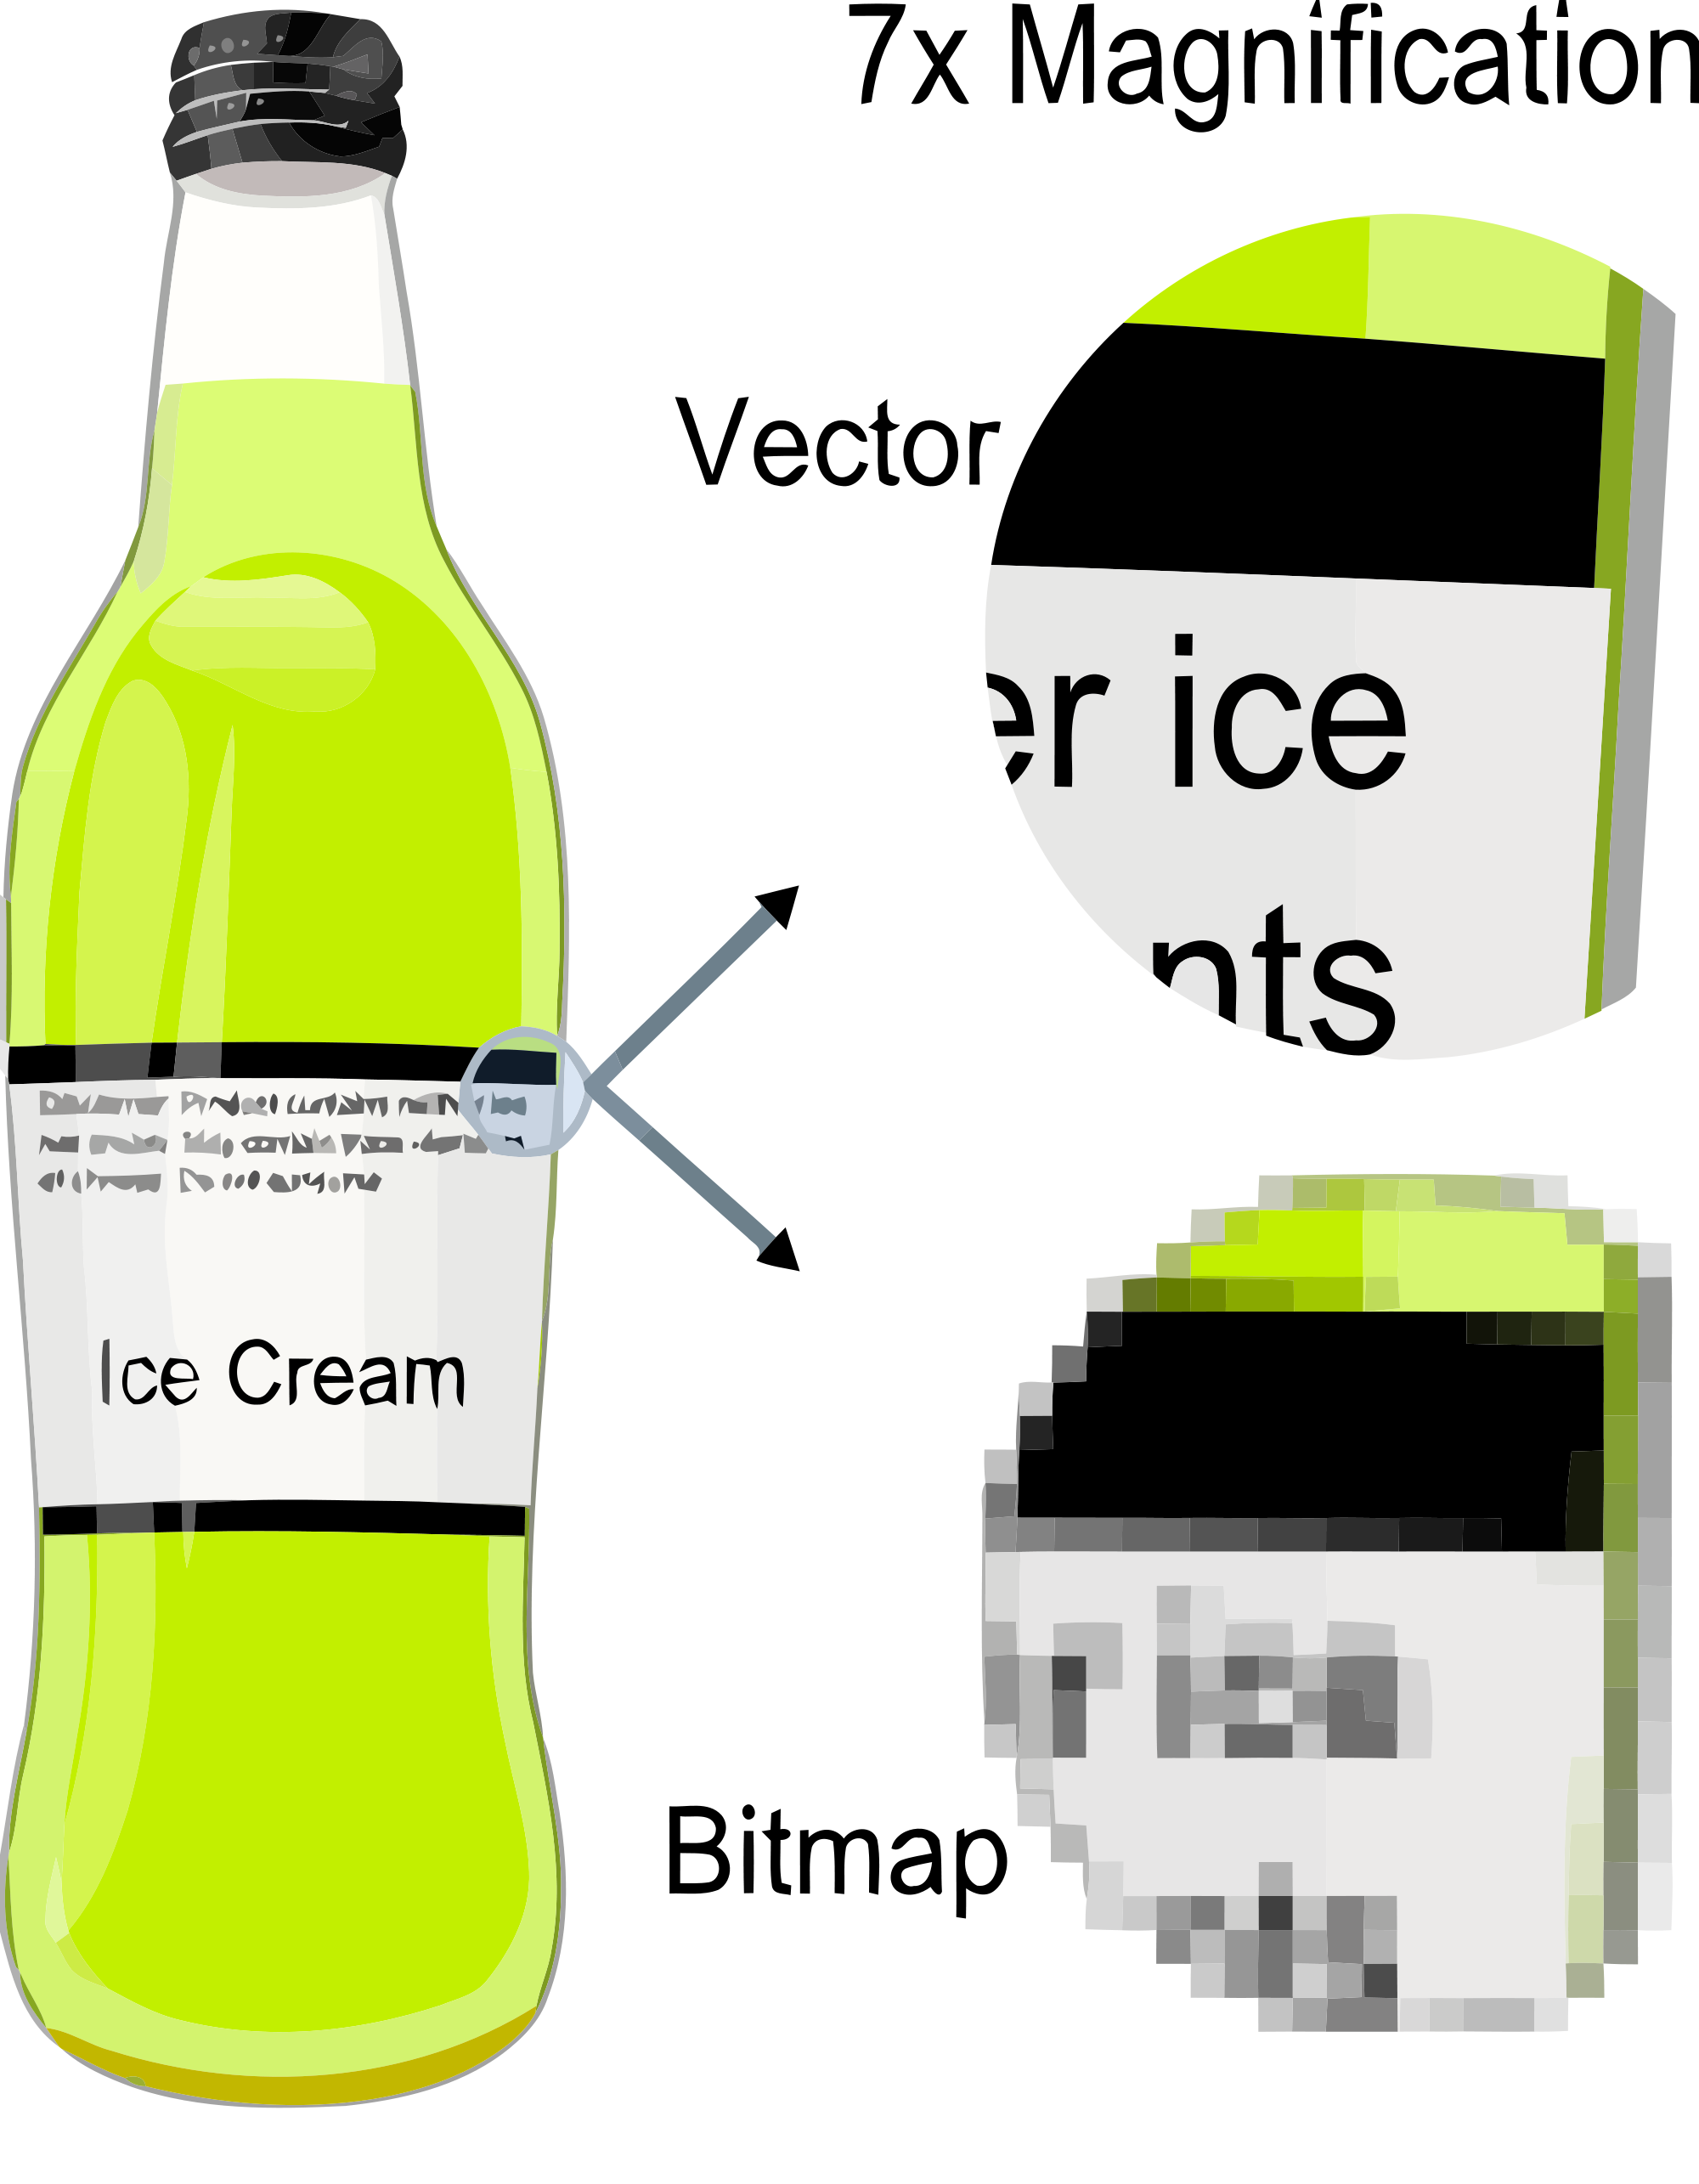
\includegraphics[height=0.7\textheight]{img/VectorBitmapExample.png}
\end{center}
\vfill
{\footnotesize Image originally by Darth Stabro, taken from \texttt{http://en.wikipedia.org}}
\vfill
\end{frame}


%--------------- slide -------------------
\begin{frame}[fragile]
\frametitle{Graphics - Supported files}
\vfill
If you are using the \texttt{latex} compiler, the only supported graphic type is \emph{Encapsulated PostScript}: \texttt{.eps} files.
\vfill
If you are using the \texttt{pdflatex} compiler, \texttt{.jpg}, \texttt{.png}, \texttt{.pdf} and \texttt{.eps} files can be used.
\vfill
\end{frame}

%--------------- slide -------------------
\begin{frame}[fragile]
\frametitle{Graphics - insertion}
\vfill
The \texttt{{\textbackslash}includegraphics} command is used to insert an image file into your \LaTeX\ document.
\vfill
\begin{lstlisting}[style=latexsty]
	\includegraphics[opt1=val1, ..., ]{imagefile}
\end{lstlisting}
\vfill
The argument to the command is the filename of the image, relative to the folder in which the \LaTeX\ is compiled.
\vfill
\begin{lstlisting}[style=latexsty]
	\includegraphics{img/rastervsvector}
\end{lstlisting}
\vfill
\end{frame}


%--------------- slide -------------------
\begin{frame}[fragile]
\frametitle{Graphics - insertion}
\vfill
We usually supply the filename of the image \emph{without} an extension, and allow \LaTeX\ to choose which file to use. \LaTeX\ will choose the best type of image depending on the compiler and output type.
\vfill
You can specify which graphics types are to be used by including the \texttt{{\textbackslash}DeclareGraphicsExtensions} command in your preamble.
\vfill
\begin{lstlisting}[style=latexsty]
	\DeclareGraphicsExtensions{.pdf,.png,.jpg}
\end{lstlisting}
\vfill
\end{frame}


%--------------- slide -------------------
\begin{frame}[fragile]
\frametitle{\texttt{{\textbackslash}includegraphics} - options}
\vfill
\begin{tabular}{r | l}
	\texttt{width=xx} & Specify the preferred width of the image \\
  	\texttt{height=xx} & Specify the preferred height of the image \\
   	\texttt{keepaspectratio} & True or False, affects behaviour when scaling \\
    \texttt{scale=xx} & Scale the image by the given factor \\
    \texttt{angle=xx} & Rotate the image by the given number of degrees \\
    \texttt{trim=l b r t} & Crop the image \\
    \texttt{clip} & Must be true for \texttt{trim} to work \\
	\texttt{page=x} & Select a particular page from a \texttt{.pdf} file\\
\end{tabular}
\vfill
\end{frame}

%--------------- slide -------------------
\begin{frame}[fragile]
\frametitle{\texttt{{\textbackslash}includegraphics} - examples}
\vfill
	\begin{LTXexample}[style=latexsty]
		
\includegraphics{img/background}
	\end{LTXexample}
\vfill
\end{frame}

%--------------- slide -------------------
\begin{frame}[fragile]
\frametitle{\texttt{{\textbackslash}includegraphics} - scale}
\vfill
We can scale an image by a given factor
\vfill
	\begin{LTXexample}[style=latexsty]
		\begin{center}
		    
\includegraphics[scale=0.25]{img/background}
		\end{center}
	\end{LTXexample}
\vfill
\end{frame}

%--------------- slide -------------------
\begin{frame}[fragile]
\frametitle{\texttt{{\textbackslash}includegraphics} - width}
\vfill
We can set the image to a preferred width
\vfill
	\begin{LTXexample}[style=latexsty]
		\begin{center}
		    
\includegraphics[width=4cm]{img/background}
		\end{center}
	\end{LTXexample}
\vfill
\end{frame}

%--------------- slide -------------------
\begin{frame}[fragile]
\frametitle{\texttt{{\textbackslash}includegraphics} - height}
\vfill
Or we can set the image to a preferred height
\vfill
	\begin{LTXexample}[style=latexsty]
		\begin{center}
		    
\includegraphics[height=4cm]{img/background}
		\end{center}
	\end{LTXexample}
\vfill
\end{frame}

%--------------- slide -------------------
\begin{frame}[fragile]
\frametitle{\texttt{{\textbackslash}includegraphics} - width and height}
\vfill
Or we can set the image to a preferred height \emph{and} width
\vfill
	\begin{LTXexample}[style=latexsty]
		\begin{center}
		    
\includegraphics[width=4cm, height=2cm]{img/background}
		\end{center}
	\end{LTXexample}
\vfill
\end{frame}

%--------------- slide -------------------
\begin{frame}[fragile]
\frametitle{\texttt{{\textbackslash}includegraphics} - width and height}
\vfill
Or we can set the image to a preferred height \emph{and} width, but maintain the aspect ratio.
\vfill
	\begin{LTXexample}[style=latexsty]
		\begin{center}
		    
\includegraphics[width=4cm, height=2cm, keepaspectratio=true]{img/background}
		\end{center}
	\end{LTXexample}
\vfill
\end{frame}


%--------------- slide -------------------
\begin{frame}[fragile]
\frametitle{\texttt{{\textbackslash}includegraphics} - relative width or height}
\vfill
We can set the image size relative to items in our environment such as the \texttt{{\textbackslash}linewidth}, \texttt{{\textbackslash}textwidth} or \texttt{{\textbackslash}textheight}
\vfill
	\begin{LTXexample}[style=latexsty]
		\begin{center}
		    
\includegraphics[width=\textwidth]{img/background}
		\end{center}
	\end{LTXexample}
\vfill
\end{frame}


%--------------- slide -------------------
\begin{frame}[fragile]
\frametitle{\texttt{{\textbackslash}includegraphics} - relative width or height}
\vfill
	\begin{LTXexample}[style=latexsty]
		\begin{center}
		    
\includegraphics[width=0.5\textwidth]{img/background}
		\end{center}
	\end{LTXexample}
\vfill
\end{frame}

%--------------- slide -------------------
\begin{frame}[fragile]
\frametitle{\texttt{{\textbackslash}includegraphics} - rotating}
\vfill
	\begin{LTXexample}[style=latexsty]
		\begin{center}
		    
\includegraphics[width=0.4\textwidth, angle=90]{img/background}
		\end{center}
	\end{LTXexample}
\vfill
\end{frame}

%--------------- slide -------------------
\begin{frame}[fragile]
\frametitle{\texttt{{\textbackslash}includegraphics} - trim}
\vfill
We can crop parts of the image off the \texttt{\textbf{l}eft}, \texttt{\textbf{b}ottom}, \texttt{\textbf{r}ight} or \texttt{\textbf{t}op}
\vfill
	\begin{LTXexample}[style=latexsty]
		\begin{center}
		    
\includegraphics[trim= 10mm 60mm 80mm 5mm, clip, width=0.4\textwidth]{img/background}
		\end{center}
	\end{LTXexample}
\vfill
\end{frame}


%--------------- slide -------------------
\begin{frame}[fragile]
\frametitle{Graphics - borders}
\vfill
The \texttt{{\textbackslash}fbox} command can be used to put borders around things like pictures
\vfill
	\begin{LTXexample}[style=latexsty]
		\begin{center}
		    \fbox{
\includegraphics[width=0.4\textwidth]{img/background}}
		\end{center}
	\end{LTXexample}
\vfill
\end{frame}

%--------------- slide -------------------
\begin{frame}[fragile]
\frametitle{Graphics - borders}
\vfill
The border padding can be changed using the \texttt{{\textbackslash}setlength{\textbackslash}fboxsep} command
\vfill
	\begin{LTXexample}[style=latexsty]
		\begin{center}
		    \setlength\fboxsep{0pt}
		    \fbox{
\includegraphics[width=0.4\textwidth]{img/background}}
		\end{center}
	\end{LTXexample}
\vfill
\end{frame}


%--------------- slide -------------------
\begin{frame}[fragile]
\frametitle{Graphics - borders}
\vfill
The border thickness can be changed using the \texttt{{\textbackslash}setlength{\textbackslash}fboxrule} command
\vfill
	\begin{LTXexample}[style=latexsty]
		\begin{center}
		    \setlength\fboxrule{4pt}
		    \fbox{
\includegraphics[width=0.4\textwidth]{img/background}}
		\end{center}
	\end{LTXexample}
\vfill
\end{frame}

%--------------- slide -------------------
\begin{frame}[fragile]
\frametitle{Exercise 4}
\vfill
Experiment with adding images into your documents.
\vfill
\end{frame}


%--------------- slide -------------------
\begin{frame}
\frametitle{Help?}
\vfill
There are \emph{many}, \emph{many} places to get more help with \LaTeX. 
\vfill
If you have a problem, use Google! Often that will lead you straight to the documentation for the package or command you have a problem with.
\vfill
Otherwise, StackExchange has a thriving \TeX\ community where you can ask for help and advice: 
\begin{center}
	\texttt{http://tex.stackexchange.com}
\end{center}
\vfill
\end{frame}

\end{document}